\section{Krauszzerlegungen und die Erd\H{o}s--Faber--Lov\'asz Vermutung}
\subsection{Die Erd\H{o}s--Faber--Lov\'asz Vermutung}
\label{sec:EFL-Vermutung}
Der Hauptteil dieser Bachelorarbeit befasst sich mit einer neuen Herangehensweise an die Erd\H{o}s--Faber--Lov\'asz Vermutung. 
Es bezeichne $\cE(n)$ die Klasse aller Graphen welche die Vereinigung von $n$ kantendisjunkten vollst"andigen Graphen der Ordnung $n$ sind. 

\begin{figure}[htbp]
        \centering
        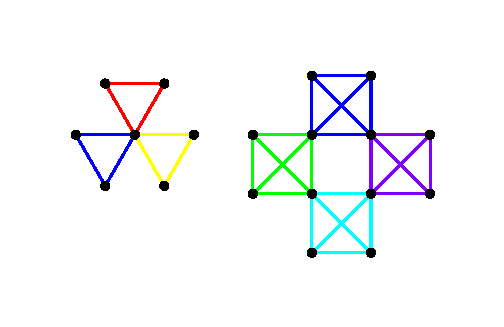
\includegraphics{images/bildeg3und4}
        \caption{Zwei Graphen aus $\cE(3)$ und $\cE(4)$}
        \label{fig:egraphen}
\end{figure}

F"ur $G\in\cE(n)$ gilt also $G= \bigcup\limits_{i=1}^{n} G_i$, wobei $G_i \cong K_n$ und $|G_i \cap G_j| \leq 1$ f"ur alle $1\leq i,j \leq n$ mit $i\neq j$ (in Abbildung \ref{fig:egraphen} sind die Kanten der vollst"andigen Graphen mit der selben Farbe markiert).
\begin{conjecture}[Erd\H{o}s--Faber--Lov\'asz(1972)]
  Sei $G\in\cE(n)$. Dann ist $\chi(G) = n$.
  \label{con:efl}
\end{conjecture}
"Uber diese Vermutung ist viel bekannt, ein vollst"andiger Beweis fehlt jedoch bis jetzt. Wir wollen nun einige bekannte Resultate beziehungsweise "aquivalente Formulierungen dieser Vermutung angeben. Im Anschluss werden wir eine Vermutung "uber den $k$-ten Eigenwert $k$-chromatischer Graphen aufstellen, welche (sollte sie sich als wahr herausstellen) Vermutung \ref{con:efl} impliziert.
\begin{remark}
  Vermutung \ref{con:efl} gilt f"ur $n\leq 10$.
\end{remark}
\todo{Quelle}
\subsection{Krauszzerlegungen von Graphen}
Die Graphen aus $\cE(n)$ lassen sich alle durch $n$ vollst"andige Graphen der Ordnung $n$ kantendisjunkt "uberdecken. Im Folgenden wollen wir ein allgemeineres Konzept betrachten, indem wir nicht fordern, dass alle Graphen der "Uberdeckung die selbe Ordnung haben. 
Diese Art der "Uberdeckung wurde zuerst von Krausz zur Charakterisierung von Kantengraphen verwendet, daher der Name Krauszzerlegung.
\todo{ausf"uhrlicher}
\label{ssec:Krauszzerlegung}
\begin{definition}
  \label{def:Krauszzerlegung}
  Sei $G$ ein Graph. Eine Menge $\mathcal K$ von Untergraphen von $G$ hei"st \DF{Krauszzerlegung} von $G$, falls folgende Bedingungen erf"ullt sind:
  \begin{enumerate}[label={\rm(K\alph*)}]
    \item Alle Graphen $K\in \mathcal{K}$ sind vollst"andige Graphen mit $|K| \geq 2$.
    \item Sind $K,K'$ zwei verschiedene Graphen aus $\mathcal{K}$, so sind sie kantendisjunkt 

      (d.h. $|K\cap K'| \leq 1$)
    \item $\mathcal K$ ist eine "Uberdeckung von $G$, d.h.  $G=\bigcup\limits_{K\in \mathcal K}K$
  \end{enumerate}
  Desweiteren sei f"ur $v\in V(G)$ der \DF{Grad} von $v$ bez"uglich $\mathcal K$ definiert als $$d_G(v:\mathcal K) = |\{ K\in\mathcal K| v \in V(K)\}|$$ und der \DF{Minimalgrad} von $G$ bez"uglich $\mathcal K$ als $$\delta_G(\mathcal K) = \min\limits_{v\in V(G)}d_G(v:\mathcal K)$$ 
  F"ur $d \geq 1$ sei $\kappa_d(G)$ die kleinste positive Zahl $m$ derart, dass $G$ eine Krauszzerlegung $\mathcal K$ mit $|\mathcal K| = m$ und $\delta_G(\mathcal K) \geq d$ besitzt. Existiert keine solche Zahl $m$, so setzen wir $\kappa_{d}(G) = \infty$.
\end{definition}

\begin{example}
  \begin{figure}[htb]
    \centering
    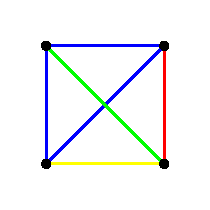
\includegraphics{images/krauszzerlegungk4.eps}
    \caption{Eine Krauszzerlegung des $K_4$}
    \label{fig:KrauszzerlegungK4}
  \end{figure}
  In Abbildung \ref{fig:KrauszzerlegungK4} sehen wir eine Krauszzerlegung $\mathcal{K}$ des $K_4$ (die einzelnen kantendisjunkten Untergraphen sind jeweils mit der selben Farbe markiert). Wir k"onnen au{\ss}erdem erkennen, dass $\delta_{G}(\mathcal{K}) = 2$, und folglich $\kappa_{2}(K_4) \leq 4$ (wir werden sp"ater sehen, dass $\kappa_{2}(K_n) \geq n$ stets gilt, und somit $\kappa_{2}(K_{4}) = 4$ ist). 
\end{example}
\begin{lemma}
  Seien $G$ ein Graph und $d\in \N$. Genau dann ist $\kappa_{d}(G) < \infty$, wenn $\delta(G) \geq d$ ist. \label{lm:krauszexistenz}
\end{lemma}
\begin{proof}
  Wir zeigen zun"achst, dass $\delta(G) \geq d$ ist, falls $p = \kappa_d(G) < \infty$. Sei $v\in V(G)$ mit $d_{G}(v) = \delta(G)$. Dann existiert eine Krauszzerlegung $\mathcal{K}=\left\{ K^{1}, \dots , K^{p} \right\}$ von $G$ mit $\delta_{G}(\mathcal{K}) \geq d$. Da alle Graphen der Krauszzerlegung kantendisjunkt sind, gilt $$ d \leq \sum\limits_{K\in \mathcal{K}, v\in K} d_{K}(v) \leq d_{G}(v) = \delta(v).$$
  Dabei gilt die erste Ungleichung, da $v$ in mindestens $d$ der Graphen aus $\mathcal{K}$ vorkommt.

  Sei nun $\delta(G) \geq d$. Wir m"ussen zeigen, dass es eine Krauszzerlegung $\mathcal{K}$ gibt, mit
  $d_{G}(v:\mathcal{K}) \geq d$ f"ur alle $v\in V(G)$. Sei $E(G)= \{e_1,\dots, e_{m}\}$ eine Nummerierung der Kanten. Sei dann $K^i$ der Graph, welcher nur aus der Kante $e_i$ und den zu $e_i$ inzidenten Kanten besteht. Wir zeigen: $\mathcal{K} = \left\{ K^i | 1 \leq i \leq m \right\}$ ist eine Krauszzerlegung von $G$ mit $\delta_{G}(\mathcal{K}) \geq d$. (Ka) ist trivialerweise erf"ullt, da alle Graphen von $\mathcal{K}$ isomporph zu $K_{2}$ sind. Sind $K,K'$ zwei verschiedene Graphen aus $\mathcal{K}$, so sind sie
  kantendisjunkt, da ihre einzigen Kanten in $G$ verschieden sind. Also ist auch (Kb) erf"ullt. Da jede Kante von $G$ in einem $K\in \mathcal{K}$ vorkommt, ist auch (Kc) erf"ullt. Sei nun $v$ eine Ecke von $G$. Dann ist $$d_{G}(v:\mathcal{K}) = d_{G}(v) \geq \delta(G) \geq d$$ und folglich auch $\delta_{G}(\mathcal{K}) \geq d$. Damit ist gezeigt, dass $\mathcal{K}$ eine Krauszzerlegung von $G$ ist mit $\delta_{G}\left( \mathcal{K} \right) \geq d$. Also ist $\kappa_{d}(G) \leq |K| <
  \infty$.
\end{proof}

\begin{example}
  Sei $G$ ein dreiecksfreier Graph mit Minimalgrad mindestens $d$. Dann ist $\kappa_{d}(G) = |E(G)|$, da $G$ keine Dreiecke enth"alt und somit jeder Graph einer Krauszzerlegung von $G$ isomorph zu $K_{2}$ sein muss. 
\end{example}

%\begin{lemma}
%  Sei $H$ ein linearer Hypergraph mit $|e| \geq d$ f"ur alle $e \in E(H)$ und ein $d \geq 2$. Sei $E_{H}(v)$ die Menge aller Kanten von $H$, welche $v$ enthalten, und $K^{v} = G[E_{H}(v)]$. Dann ist $\mathcal{K}= \left\{ K^{v}| v \in V(H), |E_{H}(v)| \geq 2 \right\}$ eine Krauszzerlegung von $G$ mit $\delta_{G}(\mathcal{K}) \geq d$. 
%  \label{lm:hyperkrausz}
%\end{lemma}
%
%\begin{proof}
%  Wir zeigen zun"achst, dass $\mathcal{K}$ eine Krauszzerlegung ist. 
%  Sei $v\in V(H)$ mit $|E_{H}(v)| \geq 2$ beliebig, wir m"ussen nun zeigen, dass $K^{v}$ ein vollst"andiger Graph der Ordnung mindestens $2$ ist. Seien $e,e' \in V(K^{v}) = E_H (v)$. Dann ist $e\cap e' = \left\{ v \right\}$ und folglich $ee' \in E(K^{v})$. Also ist $K^{v} $ ein vollst"andiger Graph. Da $|K^{v}| = |E_H(v)| \geq 2$ f"ur $K^{v}\in \mathcal{K}$ ist (Ka) erf"ullt. Seien nun $K^{v}$ und $K^{w}$ zwei verschiedene Elemente von $\mathcal{K}$. 
%  Wir m"ussen zeigen, dass diese kantendisjunkt sind. Angenommen, dem ist nicht so. Dann ist $|K^{v}\cap K^{w}| \geq 2$ und folglich gibt es in $H$ zwei Kanten $e,e'$, welche sowohl $v$ als auch $w$ enthalten, ein Widerspruch zur Vorraussetzung, dass $H$ ein lineare Hypergraph ist. Folglich ist (Kb) erf"ullt. 
%  Sei $e\in E(H) = V(G)$ eine Ecke von $G$. 
%\end{proof}
\begin{theorem}
  Die folgenden Aussagen sind "aquivalent:
  \begin{enumerate}[label={\rm(\alph*)}]
    \item F"ur alle $p\in\N$ und alle $G\in\cE(p)$ gilt $\chi(G) = p$.
    \item F"ur alle Graphen $G$ gilt $\chi(G) \leq \kappa_{2}(G)$.
    \item F"ur alle linearen Hypergraphen $H$ gilt $\chi'(H) \leq |H|$.
  \end{enumerate}
  \label{thm:equivefl}
\end{theorem}

\begin{proof}
  Wir zeigen zun"achst, dass (b) aus (a) folgt. Sei $G$ ein Graph der Ordnung $n$. Ist $\kappa_{2}(G) = \infty$, so ist nichts zu zeigen. Andernfalls ist $\kappa_{2}(G) =p$. Dann existiert eine Krauszzerlegung $\mathcal{K} = \left\{ K^1,\dots K^p \right\}$ von $G$ mit $\delta_G(\mathcal{K}) \geq 2$. Ist $p \geq n$, so gilt:
  \begin{align*}
    \chi(G) \leq n \leq p = \kappa_2 (G).
  \end{align*}
  Ist andererseits $p< n $, so ist $|K^{i}| \leq \omega (G)  \leq \kappa_2 (G) =  p$ f"ur alle $1\leq i \leq p$ (die letzte Ungleichung wird sp"ater in \ref{cor:alphaomegakrausz} gezeigt). Damit k"onnen wir f"ur $1\leq i \leq p$ jeden $K^{i}$ durch Hinzuf"ugen von Ecken und Kanten zu einem vollst"andigen Graphen vom Grad $p$ aufbl"ahen. Den so enstehenden Graphen nennen wir $G'$. Offenbar ist $G$ ein Untergraph von $G'$ und $G'\in \cE(p)$. Damit gilt 
  \begin{align*}
    \chi(G) \leq \chi (G') = p = \kappa_{2}(G)
  \end{align*}
  Also folgt (b) aus (a).  

  Um zu zeigen, dass (a) aus (b) folgt, sei $G\in \cE(p) $ mit $p\in \N$. Dann ist $G$ die kantendisjunkte Vereinigung von $p$ vollst"andigen Graphen der Ordnung $p$, welche wir mit $K^{1},\dots, K^{p}$ bezeichnen wollen. Nun entfernen wir wiederholt Ecken aus $G$,  deren aktueller Grad kleiner als $p$ ist solange, bis keine Ecken vom Grad kleiner als $p$ existieren. Den daraus resultierenden (m"oglicherweise leeren) Graphen nennen wir $H$. 
  Gelingt es, $H$ mit $p$ Farben zu f"arben, so k"onnen wir diese F"arbung schrittweise zu einer F"arbung von $G$ erweitern, indem wir die entfernten Ecken in umgekehrter Reihenfolge f"arben. Dies ist mit $p$ Farben m"oglich, da jede zu f"arbende Ecke h"ochstens $p-1$ bereits gef"arbte Nachbarn besitzt.
  Somit reicht es zu zeigen, das $\chi(H) \leq p$. Ist $V(H) =\emptyset$, so gilt dies trivialerweise. Andernfalls gilt nach Konstruktion $\delta(H) \geq p $. 
  Bleiben Ecken "ubrig, so nennen wir den resultierenden Graphen $H$. Nach Konstruktion gilt $\delta(H) \geq p$. Sei $\hat{K}^i = K^{i} \cap H$ f"ur $1\leq i \leq n$. Dann ist $\hat{K}^i$ ein vollst"andiger Graph f"ur alle $i$. W"ahle $\mathcal{K} = \left\{ \hat{K}^i | | \hat{K}^i| \geq 2  \right( , 1\leq i \leq n\}$. Wir zeigen, dass $\mathcal{K}$ eine Krauszzerlegung von $H$ mit $\delta_{H}(\mathcal{K}) \geq 2$ ist.
  Die Bedingung (Ka) ist offensichtlich erf"ullt. Da in $G$ die $K^{i}$ kantendisjunkt sind, sind die $\hat{K}^{i}$ in $H$ ebenfalls kantendisjunkt. Folglich ist die Bedingung (Kb) ebenfalls erf"ullt. Sei $v\in V(H)$. Dann ist $d_{H}(v) \geq p$, und somit gilt $d_{G}(v) \geq d_H(v) \geq p$. 
  Die Ecke $v$ ist in mindestens zwei vollst"andigen Graphen $K$ und $K'$ aus der Krauszzerlegung $\mathcal{K}$ enthalten. 
  Ansonsten w"are $v$ nur in einem vollst"andigen Graphen $K \in \mathcal{K}$ enthalten und somit w"are $d_{H}(v) = d_{K}(v) \leq p-1$, was unm"oglich ist. 
  Folglich ist $d_{H}(v:\mathcal{K}) \geq 2$ f"ur alle $v \in V(H)$. Also ist $\mathcal{K}$ eine Krauszzerlegung mit $\delta_{H}(\mathcal{K}) \geq 2$, und wegen (b) folgt dann:
  \begin{equation*}
    \chi(H) \leq \kappa_{2}(H) \leq |\mathcal{K}| \leq p .
  \end{equation*}
  Damit ist die "Aquivalenz von (a) und (b) gezeigt. 

  Es bleibt die "Aquivalenz von (b) und (c) zu zeigen. 
  Zun"achst zeigen wir, dass (b) aus (c) folgt. Dazu betrachten wir einen beliebigen Graphen $G$ und zeigen, dass $\chi(G) \leq \kappa_{2}(G)$ gilt. Ist $\kappa_{2}(G) = \infty$, so ist (b) trivialerweise erf"ullt. Andernfalls ist $\kappa_{2}(G) = p < \infty $ und es gibt eine Krauszzerlegung $\mathcal{K}= \left\{ K^{1},\dots,K^{p} \right\}$ von $G$ mit $\delta_{G}(\mathcal{K}) \geq 2 $.  
  F"ur $v\in V(G)$ definiere $e_v$ als die Menge aller $K\in \mathcal{K}$, welche $v$ enthalten. Auf Grund der Wahl der Krauszzerlegung gilt $|e_v| = d_{G}(v:\mathcal{K})\geq \delta_{H}(\mathcal{K}) \geq 2$ f"ur alle $v \in V(G)$. Sei $H$ der Hypergraph mit Eckenmenge $\mathcal{K}$ und Kantenmenge $\left\{ e_v| v\in V(G) \right\}$. Wir betrachten $\pi: V(G) \mapsto E(H)$ mit $\pi(v) = e_v$, diese ist offensichtlich surjektiv. Wir zeigen, dass $\pi$ bijektiv ist. W"are dem nicht so, so g"abe es zwei unterschiedliche Ecken $v,w$ mit $e_v = e_w$. 
  Da $|e_v| \geq 2$ ist,  w"are dann die Kante $vw$ in zwei Graphen von $\mathcal{K}$ enthalten, was der Bedingung (Kb) widerspr"ache. Also ist $\pi$ bijektiv.
  Wir zeigen nun, dass $H$ ein linear Hypergraph ist. 
  Seien dazu $e_{v},e_{w} $ zwei unterschiedliche Kanten von $H$.
  Angenommen $|e_{v}\cap e_{w}| \geq 2$. Dies ist ein Widerspruch zu Eigenschaft (Kb) der Krauszzerlegung $\mathcal{K}$. Folglich ist $|e_{v}\cap e_{w}| \leq 1$, also ist $H$ linear. Dann folgt aus der Vorraussetzung (c), dass $\chi'(H) \leq |H| = \kappa_{2}(G)$ ist.
  Somit finden wir eine F"arbung $g : E(H) \mapsto \left\{ 1,\dots,p \right\}$ der Kanten von $H$. Sei dann $f =  g \circ \pi$. Wir zeigen, dass $f$ eine F"arbung der Ecken von $G$ ist. Dazu betrachten wir eine Kante $vw\in E(G)$. Dann existiert ein $K\in \mathcal{K}$ mit $vw\in E(K)$. Also ist $e_v\cap e_w \neq \emptyset$ und folglich \begin{equation*}
    f(v) = g(e_v) \neq g(e_w) = f(w).
  \end{equation*} 
  Also ist $f$ ein $p$-F"arbung von $G$. Das hei{\ss}
  \begin{equation*}
    \chi(G) \leq p = \kappa_{2}(G).
  \end{equation*}
  Also folgt (b) aus (c).

  Dass (c) aus (b) folgt, zeigen wir durch Widerspruch. Gelte (b) und sei $H$ ein linearer Hypergraph minimaler Ordnung welcher (c) nicht erf"ullt (d.h. ist $H'$ ein weiterer linearer Hypergraph mit $|H'| < |H|$, so ist $\chi'(H') \leq | H'|$). Ist $\delta(H) \leq 1$, so k"onnen wir aus $H$ eine Ecke $v$ mit $d_H(v) \leq 1$ entfernen. F"ur den Hypergraphen $H' = H - v $ gilt dann $\chi'(H') \leq |H'| = |H|-1$. Da $v$ in h"ochstens einer Kante von $H$ enthalten ist, l"asst sich die F"arbung
  von $H'$ zu einer $\chi'(H) +1$-F"arbung von $H$ erweitern.
  Dies steht im Widerspruch zur Wahl von  $H$.  Also ist $\delta(H) \geq 2$. Sei $G$ der Kantengraph von $H$, d.h. $V(G) = E(H)$ und $E(G) = \left\{ ee'|e\cap e' \neq \emptyset, e,e' \in E(H) \right\}$. F"ur $v\in V(H)$ seien $E_{H}(v) = \left\{ e \in E(H) | v\in e \right\}$ und $K^{v} = G[E_H(v)]$.
  Wir zeigen, dass die Menge $\mathcal K = \left\{ K^{v}| v \in V(H) \right\}$ eine Krauszzerlegung von $G$  mit $\delta_{G}(\mathcal{K}) \geq 2$ ist.
  Sei also $K \in \mathcal{K} $ beliebig. Dann gibt es eine Ecke $v\in V(H)$ mit $K = K^{v} = G[E_{H}(v)]$. Seien weiterhin $e,e' \in E_H(v)$ unterschiedliche Kanten. Da $H$ ein linearer Hypergraph ist, ist $e\cap e' = \left\{ v \right\}$ und deswegen $ee'\in E(K^{v})$. Also ist $K^{v}$ ein vollst"andiger Graph.
  Au{\ss}erdem ist \begin{equation*}
    |K^{v}| = |E_{H}(v)|= d_{H}(v) \geq \delta(H) \geq 2
  \end{equation*}
  Also erf"ullt $\mathcal{K}$ die Bedingung (Ka). Seien nun $K^{v},K^{w}$ zwei verschiedene vollst"andige Graphen aus $\mathcal{K}$. Wir m"ussen zeigen, dass diese keine Kante in $G$ gemeinsam haben. Angenommen, es g"abe eine solche Kante $ee'\in E(G)$. Dann w"are $v,w \in e \cap e'$. Ein Widerspruch, da $H$ ein linearer Hypergraph ist. Also erf"ullt  $\mathcal{K}$ (Kb). Sei $ee'\in E(G)$. Folglich ist $e\cap e' \neq \emptyset$ und es existiert eine Ecke $v$ von $H$ mit $e \cap e ' = \left\{ v
  \right\}$ (da $H$ linearer Hypergraph). Damit sind $e,e'\in V(K^{v})$. Da $K^{v}$ ein vollst"andiger Graph ist, ist $ee'\in E(K^{v}$. Also erf"ullt $\mathcal{K}$ die Bedingung (Kc). 
  Es bleibt zu zeigen, dass $\delta_{G}(\mathcal{K}) \geq 2$ ist. Sei dazu $e \in V(G)$ beliebig. Da wir $H$ als schlingenlos angenommen haben, existieren zwei unterschiedliche Ecken $v,w \in e$. Also ist $e\in K^{v}$ und $e\in K^{w}$. Diese beiden vollst"andigen Graphen sind unterschiedlich, da sonst $v$ und $w$ in zwei Kanten enthalten sind. \todo{Genauer!} Das ist aber unm"oglich, da $H$ ein linearer Hypergraph ist. 
  Damit ist \begin{equation*}
    \chi'(H) = \chi(G) \leq \kappa_{2}(G) \leq |\mathcal{K}| = |H|
  \end{equation*}
  Ein Widerspruch zur Annahme $\chi'(H) > |H|$.
\end{proof}
\subsection{Krauszzerlegungen und Eigenwerte}

\begin{theorem}
  \label{thm:KrauszEigenwerte}
  Seien $G$ ein Graph mit $V(G)=\{v_1,\dots,v_n\}$ und $\mathcal K=\{K^1,\dots,K^p\}$ eine Krauszzerlegung von $G$ mit $d_G(\mathcal K) \geq d \geq 2$ . Desweiteren sei $d_i = d_G(v_{i}:\mathcal K)$ f"ur $1\leq i \leq n$. 
  Dabei w"ahlen wir die Eckennummerierung so, dass $d_1 \geq \dots \geq d_{n}$ ist.
  Dann gelten folgende Aussagen : 
  \begin{enumerate}[label=\rm{(\alph*)}]
    \item $\lambda_i(G) \geq -d_{n-i+1}$ f"ur $i = 1, \dots , n$.
    \item $\lambda_{p+1}(G) \leq -d$ falls $p < n$ ist.
  \end{enumerate}
\end{theorem}
\begin{proof}
  Zun"achst zeigen wir (a). Es sei $A$ die Adjazenzmatrix von $G$ und $D := \operatorname{diag}(d_1,\dots,d_n)$. Definiere $B\in\R^{n\times m}$ als die Inzidenzmatrix von $\mathcal K$, also $$B_{i,j} = \begin{cases}
    1 & v_i \in K^j \\ 0 & v_i \notin K^j
  \end{cases}$$ 
  Nun betrachten wir $M=BB^{T}$. Es gilt
  \[
    M_{i,j} = \sum\limits_{k=1}^{d}B_{i,k}B_{j,k}
  \]
  Seien zun"achst $i,j \in \{1,\dots,n\}$ mit $i\neq j$. Ist $B_{i,k} = 1$ und $B_{j,k} = 1$, so ist $v_i,v_j  \in K^k$, und somit (da $K^k$ ein vollst"andiger Graph ist) $v_iv_j\in E(G)$. Es k"onnen aber f"ur h"ochstens ein $k\in \{1,\dots,m\}$ $B_{i,k}$ und $B_{j,k}$ gleichzeitig $1$ seien, da nach Definition \ref{def:Krauszzerlegung} die Graphen aus $\mathcal K$ kantendisjunkt sind. Also ist $M_{i,j}= 1 $ genau dann, wenn $v_iv_j\in E(G)$, genau dann wenn $A_{i,j} = 1$. Somit ist $M_{i,j}=A_{i,j}$\\
  Sei nun $i\in\{1,\dots,n\}$ beliebig. Wir betrachten $M_{i,i}$. Es gilt 
  \[
    M_{i,i} = \sum\limits_{k=1}^{d}B_{i,k}B_{i,k} = \sum\limits_{k=1}^{d} B_{i,k}.
  \]
  $B_{i,k}=1$ gilt genau dann, wenn $v_i \in K^k$. Folglich ist $M_{i,i}= d_G(v_i:\mathcal K)= d_i$. Damit gilt $M=A+D$. $M$ ist nach Satz \ref{prop:psdmatrix} positiv semidefinit.
  Folglich ist $A- (-D)$ positiv semidefinit, und es folgt mit Lemma \ref{lem:evpsddif}, dass 
  \begin{equation*}
    \lambda_i(G) = \lambda_i(A) \geq \lambda_i(-D) = -d_{n-i+1}
  \end{equation*}
  Damit ist (a) gezeigt.

  Nun zeigen wir (b). Sei $p<n$. Dann ist $\operatorname{rang}(M)= \operatorname{rang}(B) \leq p$. Also ist $\lambda_{p+1}(M) = 0$ und es folgt mit Satz \ref{thm:weylineq} dass 
  \begin{align*}
    \lambda_{p+1}(A) + d \leq \lambda_{p+1}(A) + d_{n} \leq 0
  \end{align*}
  Durch Umstellen erhalten wir die gew"unschte Ungleichung.
\end{proof}
\begin{corollary}
  \label{cor:Korollar1}
  Sei $H$ ein induzierter Untergraph von $G$ und seien $q,d \in \N$ mit $q \leq |H|$ und $d \geq 2$.
  Ist $\lambda_{q}(H) \geq -d$, so ist $\kappa_{d}(G) > q$.
\end{corollary}
\begin{proof}
  Angenommen es gilt $p = \kappa_{d}(G) < q$. Dann gibt es  eine Krauszzerlegung $\mathcal{K}$ von $G$ mit $|\mathcal{K}| = p$ und $\delta_G(\mathcal{K}) \geq d$. Wegen Lemma \ref{lem:InterlacingGraphen} gilt dann $\lambda_{q}(G) \geq \lambda_{q}(H) > -d $. Andererseits folgt aus Satz \ref{thm:KrauszEigenwerte} dass $\lambda_{q}(G) \leq \lambda_{p+1} \leq -d $, ein Widerspruch. 
\end{proof}

\begin{corollary}
  \label{cor:LineGraphWald}
  Seien $\delta(G) \geq 2$ und $H$ ein induzierter Untergraph von $G$. Ist $H$ Kantengraph eines Waldes, so gilt 
  Dann ist $\kappa_{2}(G)\geq \left|H\right|$.
\end{corollary}

\begin{proof}
  Sei $q = |H|$. Da $H$ Kantengraph eines Waldes ist, folgt $\lambda_{q}(H) > -2$ (vgl. \cite[3.4.10]{zbMATH05625877}) 
  Dann ist mit Korollar \ref{cor:Korollar1} $\kappa_{2}\left( G \right) \geq \left| H\right|$.
\end{proof}

\begin{corollary}[Klotz]
  $\kappa_{2}\left( K_n \right) \geq n$
\end{corollary}

\begin{proof}
  $K_n$ ist der Kantengraph von $K_{1,n}$. Nun folgt die Behauptung aus Korollar \ref{cor:LineGraphWald}.
\end{proof}
\begin{corollary}
  Ist $\delta\left( G \right) \geq 2$, so gilt $\omega\left( G \right)\leq \kappa_{2}\left( G \right)$ und $\alpha\left( G \right)\leq \kappa_{2}\left( G \right)$.
  \label{cor:alphaomegakrausz}
\end{corollary}

\begin{proof}
  Sei $p = \omega(G)$. Dann gilt nach Korollar \ref{cor:alphaomegaEigenwerte} $\lambda_{p}\left( G \right)\geq -1 > -2$. Damit sind f"ur $d=2$ die Voraussetzungen von Korollar \ref{cor:Korollar1} erf"ullt, und es gilt folglich $\kappa_{2}\left( G \right)\geq p = \omega\left( G \right)$ .
  F"ur $q=\alpha\left( G \right)$ gilt mit Korollar \ref{cor:alphaomegaEigenwerte} $\lambda_{q}\left( G \right)\geq 0 > -2$. Damit folgt $\alpha\left( G \right) \leq \kappa_{2}\left( G \right)$.
\end{proof}

\begin{theorem}
  \label{thm:MainTheorem}
  Existiert ein $d\in \N$, sodass f"ur alle  Graphen $G$ mit $\chi(G) = k $ gilt $ \lambda_{k}(G) > -d$. Dann gelten folgende Aussagen:
  \begin{enumerate}[label=(\alph*)]
    \item F"ur alle Graphen $G$ gilt $\chi(G) \leq \kappa_d (G)$.
    \item  Ist $H$ ein linearer Hypergraph mit $\left|e\right| \geq d$ f"ur alle $e\in E(H)$, so ist $\chi'\left( H \right)\leq \left|H\right| $
  \end{enumerate}
\end{theorem}

\begin{proof}
  Wir zeigen zun"achst (a). Sei $G$ ein beliebiger Graph mit $\chi(G) = k$. Nach Voraussetzung des Satzes ist dann $\lambda_{k}\left( G \right) > -d$. Mit Korollar \ref{cor:Korollar1} folgt $\kappa_{d}\left( G \right) \geq k = \chi\left( G \right)$. 
  Damit ist (a) gezeigt. 

  Wir zeigen nun (b) durch Widerspruch. Angenommen die Behauptung gilt nicht. Dann gibt es einen linearen Hypergraphen minimaler Ordnung mit $|e| \geq d$ f"ur alle $e\in E(H)$ , f"ur welchen $\chi'(H) > H$. 
  \todo{fallunterscheidung}
  Fall 1: Es existiert eine Kante $e$ von $H$ vom Grad kleiner als $d$. Da $|e| \geq d$ ist und $H$ ein linearer Hypergraph ist, gibt es eine Ecke $v$ von $H$ welche nur in $e$ vorkommt. Diese entfernen wir und erhalten einen Hypergraphen $H'$ der Ordnung $|H'| = |H|-1$. Dieser l"asst sich mit $\chi'(H') \leq |H'|$ Farben f"arben. Diese F"arbung k"onnen wir zu einer F"arbung von $H$ mit h"ochstens $|H'|+1 = |H|$ Farben erweitern. Ein Widerspruch zur Wahl von $H$.

  Fall 2: Alle Kanten von $H$ haben mindestens den Grad $d$. 

  Angenommen in diesem exisitiert eine Kante vom Grad kleiner als $d$. Entfernen wir diese, erhalten wir einen Hypergraphen $H'$ kleinerer M"achtigkeit.
  Dieser erf"ullt die Behauptung, da $H$ das kleinste Gegenbeispiel ist. Also existiert eine Kantenf"arbung von $H'$ mit h"ochstens $|H'| < |H|$ Farben. Aus dieser gewinnen wir eine Kantenf"arbung von $H$, indem wir alle Kanten wie in $H'$ f"arben, und die entfernte Kante mit einer neuen Farbe f"arben. Folglich gilt also:
  \begin{align*}
    \chi'(H) \leq \chi'(H') +1 \leq |H'|+1 \leq |H|
  \end{align*}
  Ein Widerspruch. Folglich haben alle Kanten in $H$ mindestens Grad $d$. 

  Sei nun $G=L(H)$ der Kantengraph von $H$. Dann ist $\delta(G) \geq d$. F"ur eine Ecke  $v\in V(H)$ sei (analog zum Beweis von  Satz \ref{thm:equivefl}) $E_{H}(v) = \left\{ e\in E(H) | v\in e \right\}$ und $K^{v} = G[E_{H}(v)]$. Wie in Satz \ref{thm:equivefl} folgt, dass $\mathcal{K}=\left\{ K^{v} | v \in V(H) \right\}$ eine Krauszzerlegung von $G$ mit $\delta_{G}(\mathcal{K}) \geq d$ ist. Damit gilt
  \begin{equation*}
    \chi'(H) = \chi(G) \leq \kappa_{d}(G) \leq |\mathcal{K}| = |H|
  \end{equation*}
  Wobei die erste Ungleichung wegen (a) gilt. Damit ist alles gezeigt. 
\end{proof}


\subsection{Schranken f"ur $\kappa_d(G)$}

Wir wollen nun einige Schranken f"ur $\kappa_{d}(G)$ angeben. 
\begin{lemma}
  Ist $\delta(G) \geq d$, so ist $\kappa_{d}(G) \leq |E(G)|$. 
\end{lemma}
\begin{proof}
  Dies folgt unmittelbar aus dem Beweis von Lemma \ref{lm:krauszexistenz}. 
\end{proof}

\begin{theorem}
  Sei $G$ ein Graph der Ordnung $n$ und $d\in \N$. Dann gilt:
  \begin{align*}
    \kappa_{d}(G) &\geq \frac{nd}{\lambda_{1}(G) +d} 
    %\lambda_n(A) \leq -d 
  \end{align*}
  \label{thm:kappaineq1}
\end{theorem}

\begin{proof}
  Ist $\kappa_{d}(G) = \infty$, so ist nichts zu zeigen. \\
  \ncase{1}{$\kappa_{d}(G) \geq n$} Da $\lambda_{1}(G) \geq 0$, gilt 
  \begin{align*}
    \lambda_{1}(G) + d &\geq d \\
    1 &\geq \frac{d}{\lambda_{1}(G) + d }\\
    \kappa_{d}(G) \geq n &\geq \frac{nd}{\lambda_{1}(G)+d}
  \end{align*}
  \ncase{2}{$\kappa_{d}(G) < n$}
  Sei $\mathcal{K}$ eine Krauszzerlegung von $G$ mit $|\mathcal{K}| = \kappa_{d}(G)$ und $\delta_{G}(\mathcal{K}) \geq d$. Seien $d_{i} = d_{G}(v:\mathcal{K})$. Wir k"onnen annehmen, dass die $d_{i}$ fallend geordnet sind. Sei $B\in \R^{n\times p}$ die Adjanzenzmatrix von $\mathcal{K}$ und $M = BB^{T} = A+D$, wobei $A= A(G)$ und $D = \operatorname{diag}(d_{1},\dots,d_n)$.
  Dann ist $M$ positiv semidefinit und $\operatorname{rang} (M) \leq p = \kappa_{d}(G) < n $. Deswegen ist $\lambda_{p+1}(M) = \dots \lambda_{n}(M) = 0$. 
  Mit Satz \ref{thm:kyfanineq} folgt dann : 
  \begin{align*}
    \sum\limits_{i=1}^{n} \lambda_{i}(D) &=\sum\limits_{i=1}^{n} \lambda_{i}(A) +\sum\limits_{i=1}^{n}  \lambda_{i}(D) \\
    &=\sum\limits_{i=1}^{n} \lambda_{i}(M) =\sum\limits_{i=1}^{p} \lambda_{i}(M) \\
    &\leq \sum\limits_{i=1}^{p} \lambda_{i}(A) +\sum\limits_{i=1}^{p} \lambda_{i}(D)
  \end{align*}
  Daraus folgt 
  \begin{align*}
    (n-p) d \leq (n-p) \lambda_n(D) \leq \sum\limits_{i=m+1}^{n} \lambda_{i}(D) \leq\sum\limits_{i=1}^{p} \lambda_{i}(A) \leq p\lambda_{1}(A)
  \end{align*}
  Durch Umstellen nach $p$ erhalten wir die gew"unschte Ungleichung.
\end{proof}

\subsection{Chromatische Zahl und Eigenwerte}
Es ist nicht viel "uber den Zusammenhang der chromatischen Zahl eines Graphen, und seinen Eigenwerte bekannt. Wir wollen hier nur kurz auf zwei S"atze verweisen, die Schranken f"ur die chromatische Zahl eines Graphen in Abh"angigkeit des gr"o{\ss}ten bzw. kleinsten Eigenwerts angeben. Eine Absch"atzung nach oben ("ahnlich zu dem Brookschen Satz) gibt Wilf in \cite{wilf1967eigenvalues} an.

\begin{theorem}
  Ist $G$ ein Graph, so gilt: 
  $$\chi(G) \leq \lambda_{1}(G) +1$$
  Gleichheit tritt nur auf, falls $G$ ein vollst"ander Graph oder ein ungerader Kreis ist.
  \label{thm:wilfev}
\end{theorem}

Eine untere Schranke findet sich in \cite{Hoffmanbounds} (man beachte hierbei, dass $\lambda_{n}(G)$ negativ ist):

\begin{theorem}
  Ist $G$ ein Graph mit $|G| = n$, so gilt:
  $$\chi(G) \geq 1 - \frac{\lambda_{1}(G)}{\lambda_{n}(G)}$$
  \label{thm:Hoffmanev}
\end{theorem}

\subsection{$k$-chromatische Graphen mit $\lambda_{k} > -2$}

Gilt Satz \ref{thm:MainTheorem} f"ur $d=2$, so folgt die Erd\H{o}s--Faber--Lov\'asz Vermutung auf Grund von Satz \ref{thm:equivefl}. Im Folgenden wollen wir f"ur einige Graphenklassen folgende Vermutung "uberpr"ufen.
\begin{conjecture}
  Ist $G$ ein Graph mit $\chi(G) = k$, dann gilt $\lambda_{k}(G) > -2$. 
  \label{con:maincon}
\end{conjecture}

Ein Graph $G$ hei{\ss}t $k$-kritisch, falls $\chi(G) = k$ und $\chi(H) < k$ f"ur alle induzierten Untergraphen $H$ von $G$.
\begin{remark}
  Es reicht Vermutung \ref{con:maincon} f"ur $k$-kritische Graphen zu zeigen. 
\end{remark}

\begin{proof}
  Sei $G$ ein Graph mit $\chi(G) = k$. Dann enth"alt $G$ einen $k$-kritischen Untergraphen $H$. F"ur diesen gilt (nach Vermutung) $\lambda_{k}(H) > -2$. Nun folgt mit Satz \todo{referenz}
  \begin{equation*}
    \lambda_{k}(G) \geq \lambda_{k}(H) > -2
  \end{equation*}
  Damit gilt Vermutung \ref{con:maincon} auch f"ur $G$.
\end{proof}

Seien $v,r$ zwei nat"urliche Zahlen mit $v\geq r$. Der \DF{Kneser Graph} $K_{v:r}$ ist der Graph mit Eckenmenge $V(K_{v:r}) = \left\{ X \subset \left\{ 1,\dots v \right\} | |X| = r \right\}$ und Kantenmenge 

\parindent 0pt $E(K_{v:r}) = \left\{ XY| X,Y \in V(K_{v:r}), X \cap Y = \emptyset \right\}$. 

\parindent 15pt Es wurde gezeigt\todo{Referenz}, dass $\alpha(K_{v:r}) = \binom{v-1}{r-1}$ (falls $v >2r$) und $\chi(K_{v:r}) = v-2r+2$. Das, und  Korollar \ref{cor:alphaomegaEigenwerte} erlaubt uns Vermutung \ref{con:maincon} f"ur alle Kneser Graphen zu beweisen. 

\begin{proposition}
  Seien $k,v\in \N$ mit $k>v$ und sei $G= K_{v:r}$ ein Kneser-Graph mit $\chi(G) = k$. Dann gilt $\lambda_{k}(G) > -2$
\end{proposition}

\begin{proof}
  Wir machen eine Fallunterscheidung bez"uglich $r$. 

  \ncase{1} {$r=1$} Dann ist $G=K_{v:1}$ isomorph zu $K_v$, da alle Ecken von $G$ einelementige Teilmengen von $\left\{ 1,\dots, v \right\}$ sind, und diese alle miteinander disjunkt sind. Die Eigenwerte des $K_v$ sind alle gr"o{\ss}er als $-2$. 

  \ncase{2} {$v > 2r \geq 4 $} Sei $p = \alpha(G)$.  Dann ist $ p = \binom{v-1}{r-1}$ und folglich $ p \geq v-1$. Andererseits ist $\chi(G) = v-2r+2 < v-2$. Folglich ist $p > \chi(G)$. Mit  Korollar \ref{cor:alphaomegaEigenwerte} gilt dann \begin{equation*}
    \lambda_{k}(G) \geq \lambda_{p}(G) \geq 0 > -2
  \end{equation*}

  \ncase{3} {$2r = v $} Die Ecken von $G$ sind alle $r$-elementingen Teilmengen von $\left\{ 1,\dots,v \right\}$. Da $v=2r$ ist f"ur ein $w\in V(G)$ die einzige benachbarte Ecke ihr Komplement in $\left\{ 1,\dots,v \right\}$. Also sind die Komponenten von $G$ alle isomoprh zu $K_{2}$. Dann ist $\chi(G) = 2$ und $\omega(G) = 2$. Aus Korollar \ref{cor:alphaomegaEigenwerte} folgt dann, dass $\lambda_{2}(G) \geq -1 > -2$ ist.

  \ncase{4}{$2r > v$} Dann ist $|E(G)| = 0$, da je zwei Ecken nichtleeren Schnitt haben, und folglich ist $G$ ein leerer Graph, welcher nur den Eigenwert $0>-2$ besitzt. Insbesondere ist also auch $\lambda_{k}(G) > -2$.
\end{proof}

\begin{proposition}
  Sei $G$ ein perfekter Graph. Dann gilt f"ur $k=\chi(G)$:
  $$\lambda_{k}(G) > -2$$
\end{proposition}

\begin{proof}
  Da $G$ ein perfekter Graph ist, gilt $k = \chi(G) = \omega(G)$. Also besitzt $G$ einen vollst"andigen Graphen der Ordnung $k$ als induzierten Untergraphen. Nach \ref{cor:alphaomegaEigenwerte} ist $\lambda_{k}(G) > -2$.
\end{proof}

\begin{proposition}
  Vermutung \ref{con:maincon} gilt f"ur planare Graphen.
\end{proposition}

\begin{proof}
  Sei $G$ ein planarer Graph. Wir machen eine Fallunterscheidung nach $n = |G|$. 
  \ncase{1}{$n\leq6$}
  \todo{}

  \parindent 0pt \ncase{2}{$n \geq 7$}
  Wir zeigen, dass $\lambda_4(G) > -2$ gilt. Da alle planaren Graphen eine chromatische Zahl kleiner gleich $4$ haben, folgt dann die Behauptung.

  Nehmen wir daf"ur an, dass $\lambda_{4}(G) < -2$ gilt.
  Aus Lemma \ref{rem:evGraph} (i) folgt dann:
  \begin{equation*}
    \sum\limits_{i=1}^3 \lambda_{i}(G) = -\sum\limits_{i=4}^{n}\lambda_{i}(G) \geq 2 (n-3) = 2n-6
  \end{equation*}
  Mit Lemma \ref{rem:evGraph} (ii) folgt au{\ss}erdem:
  \begin{align*}
    \sum\limits_{i=1}^3 \lambda_{i}(G)^{2} &= 2m -\sum\limits_{i=4}^{n}\lambda_{i}(G)^{2} \\
    &\leq 2(3n-6) -4(n-3) = 2n
  \end{align*}
  Die Ungleichung folgt dabei aus der Absch"artzung der Kanten f"ur planare Graphen. Aus der Absch"atzung der $2$ und $1$ Norm folgt nun:

  \begin{align*}
    2n &\geq \lambda_{1}^{2} +\lambda_{2}^{2} +\lambda_{3}^{2}  \\ &\geq \frac{1}{3} (|\lambda_{1}| + |\lambda_2| + |\lambda_3|)^{2} \\
    &\geq \frac{1}{3}(\lambda_{1}+ \lambda_2 + \lambda_3)^{2}\\ &\geq \frac{1}{3}(2n-6)^{2}
  \end{align*}
  L"osen der entstehenden quadratischen Gleichung ergibt $n\leq 6$, ein Widerspruch.
\end{proof} 

